\documentclass[11pt]{article}
\usepackage[T1]{fontenc}
\usepackage{amsmath,amssymb,amsthm,booktabs,geometry,hyperref}
\geometry{margin=1in}
\newtheorem{proposition}{Proposition}
\title{Exact Lower-Order Certificates and a Search for Log-Concave Violations of Gaussian Complete Monotonicity}
\author{Computational research record}
\date{November 17, 2026 --- provisional during computation}
\begin{document}
\maketitle
\begin{abstract}
We describe reduced entropy-derivative formulas, constrained density families,
and a mixed-precision computational search at orders six, seven, and eight.
The formulas are independently checked against high-precision heat-convolution
finite differences. Rigorous finite-interval integration is combined with
analytic tail bounds and global convexity estimates. Exact rational sum-of-squares identities additionally yield the sharp Gaussian
lower bounds at orders six through eight under the stated analytic hypotheses.
This document is an ongoing-results record: an explicit order-46 witness is certified, while the exact minimal
order remains unresolved.
\end{abstract}
\section{Question and conventions}
Throughout, $P_t=e^{t\partial_x^2/2}$ and
$H(p)=\int_{\mathbb R}p\log p$ is Boltzmann entropy. Put
$S_m(p)=(-1)^m\left.\partial_t^mH(P_tp)\right|_{t=0}$.
The target is the smallest $m\ge6$ admitting a smooth positive probability
density with $V=-\log p$, $V''>0$ everywhere, and $S_m<0$.
Gu and Sellke~\cite{gu} disprove the unrestricted conjecture at order five
and establish existence of a log-concave violation at an unspecified order.
Zou, Fan, Gao, and Wang~\cite{zou} give an explicit log-concave family whose
signed derivative is negative for all sufficiently large orders.
The log-concave signs through order five are known~\cite{wang}.
Consequently, a certified order-six witness would establish minimality.
An order-seven or order-eight witness alone would establish only an upper bound.

\section{Scaling and exact reduced formulas}
\begin{proposition}[Scaling and Gaussian controls]
For $p_a(x)=a^{-1}p(x/a)$, $a>0$, one has $S_m(p_a)=a^{-2m}S_m(p)$.
For the centered Gaussian of variance $v$, $S_m=(m-1)!/(2v^m)$.
Thus $S_m(p)\operatorname{Var}(p)^m$ is scale invariant, whereas a
strictly positive universal lower bound for unnormalized $S_m$ is impossible.
\end{proposition}
\begin{proof}
Heat scaling gives $H(P_tp_a)=H(P_{t/a^2}p)-\log a$.
For the Gaussian, $H(P_tp)=-\tfrac12\log(2\pi e(v+t))$.
Differentiate these identities $m$ times.
\end{proof}
\begin{proposition}[Reduced derivative recurrence]
For smooth Gaussian-decaying densities with bounded higher log derivatives,
write $u_j=\partial_x^j\log p$. If $F$ is a polynomial in $u_2,u_3,\ldots$,
then $\partial_t\mathbb E_p F=\mathbb E_p\mathcal LF$, where
\[
\mathcal LF=-\frac12\sum_{i,j\ge2}F_{ij}u_{i+1}u_{j+1}
+\frac12\sum_{i\ge2}F_i\sum_{k=1}^{i-1}\binom{i}{k}u_{k+1}u_{i-k+1}.
\]
Starting with $F_2=u_2^2/2$, the polynomial $F_m=\mathcal L^{m-2}F_2$
satisfies $I_m=\mathbb E_p F_m$ and involves derivatives at most of order $m$.
\end{proposition}
\begin{proof}
The heat equation gives $\partial_t\log p=(u_2+u_1^2)/2$.
Differentiating $u_i$ gives its diffusion term, $u_1u_{i+1}$, and the
quadratic sum displayed above. Differentiating the expectation contributes
$\tfrac12\mathbb E_p\partial_x^2F$.
Integrating $\mathbb E_p(\partial_x^2F+u_1\partial_xF)=0$
eliminates the drift and combines the second-derivative terms into
$-\tfrac12\sum F_{ij}u_{i+1}u_{j+1}$. Gaussian tails justify the boundary limits.
\end{proof}
% Generated by src/derive_integrands.py. H=\int p\log p, \partial_t p=\frac12\partial_x^2p.
\paragraph{Conventions and recurrence.}
Put $u_j=\partial_x^j\log p$, $H(p)=\int_{\mathbb R}p\log p$, and $\partial_t p=\tfrac12\partial_x^2p$. Then $I_m=\mathbb E_p F_m$, where $F_1=-u_1^2/2$, $F_2=u_2^2/2$, and
\[F_{m+1}=-\frac12\sum_{i,j}\partial_{u_i}\partial_{u_j}F_m\,u_{i+1}u_{j+1}+\frac12\sum_i\partial_{u_i}F_m\sum_{k=1}^{i-1}\binom{i}{k}u_{k+1}u_{i-k+1}.\]
The sums use only $i,j\ge2$. This recurrence eliminates $u_1$ by integration by parts and uses derivatives only through $u_m$ in $F_m$. No claim of uniqueness of the reduced representative is made. Shannon entropy is $-H$ and reverses every sign.
\begin{align*}
F_{6}={}& \frac{u_{6}^{2}}{2}
\\ &{}-15 u_{4}^{3}
\\ &{}+60 u_{2}^{6}
\\ &{}+105 u_{3}^{4}
\\ &{}-600 u_{2}^{3} u_{3}^{2}
\\ &{}-15 u_{2} u_{5}^{2}
\\ &{}+150 u_{2}^{2} u_{4}^{2}
\\ &{}-60 u_{3} u_{4} u_{5}
\\ &{}+450 u_{2} u_{3}^{2} u_{4}
\end{align*}
\begin{align*}
F_{7}={}& 360 u_{2}^{7}
\\ &{}-\frac{u_{7}^{2}}{2}
\\ &{}-6300 u_{2}^{4} u_{3}^{2}
\\ &{}-2415 u_{3}^{2} u_{4}^{2}
\\ &{}-630 u_{2} u_{4}^{3}
\\ &{}-630 u_{3}^{3} u_{5}
\\ &{}-315 u_{2}^{2} u_{5}^{2}
\\ &{}+21 u_{2} u_{6}^{2}
\\ &{}+70 u_{4}^{2} u_{6}
\\ &{}+105 u_{4} u_{5}^{2}
\\ &{}+2100 u_{2}^{3} u_{4}^{2}
\\ &{}+4410 u_{2} u_{3}^{4}
\\ &{}+105 u_{3} u_{5} u_{6}
\\ &{}+9450 u_{2}^{2} u_{3}^{2} u_{4}
\\ &{}-2520 u_{2} u_{3} u_{4} u_{5}
\end{align*}
\begin{align*}
F_{8}={}& \frac{u_{8}^{2}}{2}
\\ &{}+2520 u_{2}^{8}
\\ &{}+3115 u_{4}^{4}
\\ &{}-70560 u_{2}^{5} u_{3}^{2}
\\ &{}-47880 u_{3}^{4} u_{4}
\\ &{}-17640 u_{2}^{2} u_{4}^{3}
\\ &{}-5880 u_{2}^{3} u_{5}^{2}
\\ &{}-280 u_{5}^{2} u_{6}
\\ &{}-210 u_{4} u_{6}^{2}
\\ &{}-28 u_{2} u_{7}^{2}
\\ &{}+588 u_{2}^{2} u_{6}^{2}
\\ &{}+7140 u_{3}^{2} u_{5}^{2}
\\ &{}+29400 u_{2}^{4} u_{4}^{2}
\\ &{}+123480 u_{2}^{2} u_{3}^{4}
\\ &{}-135240 u_{2} u_{3}^{2} u_{4}^{2}
\\ &{}-35280 u_{2} u_{3}^{3} u_{5}
\\ &{}-280 u_{4} u_{5} u_{7}
\\ &{}-168 u_{3} u_{6} u_{7}
\\ &{}+3920 u_{2} u_{4}^{2} u_{6}
\\ &{}+5880 u_{2} u_{4} u_{5}^{2}
\\ &{}+5880 u_{3}^{2} u_{4} u_{6}
\\ &{}+20160 u_{3} u_{4}^{2} u_{5}
\\ &{}+176400 u_{2}^{3} u_{3}^{2} u_{4}
\\ &{}-70560 u_{2}^{2} u_{3} u_{4} u_{5}
\\ &{}+5880 u_{2} u_{3} u_{5} u_{6}
\end{align*}


\section{Explicit search families}
The first family is
\[
p(x)=Z^{-1}e^{-x^2/2}\left(1+\sum_{k=1}^K a_k\cos(\omega_kx+\theta_k)\right).
\]
If $A_0=\sum|a_k|<1$ and $A_2=\sum|a_k|\omega_k^2<1-A_0$,
then $V''\ge1-A_2/(1-A_0)>0$ globally. Its normalizer is
$Z=\sqrt{2\pi}(1+\sum a_ke^{-\omega_k^2/2}\cos\theta_k)$.
We also use $p\propto\exp[-x^2/2+\sum a_k\cos(\omega_kx+\theta_k)]$,
for which $V''\ge1-A_2$.
The positive-curvature family has
\[
 V''(x)=1+\sum_k w_k e^{-(x-c_k)^2/(2s_k^2)},\qquad w_k\ge0,\ s_k>0.
\]
Two exact integrations use
$s_k\sqrt{\pi/2}(x-c_k)\operatorname{erf}((x-c_k)/(\sqrt2s_k))
+s_k^2e^{-(x-c_k)^2/(2s_k^2)}$, together with a linear tilt.
Finally, two equal-variance Gaussian components with means $\pm d$, $d<1$,
and arbitrary positive mixture weights satisfy $V''\ge1-d^2$.
These sufficient convexity restrictions define a subset of all strictly
log-concave densities; failure to find a violation in them proves no general theorem.

\section{Numerical validation and rigorous certificates}
For $p(x)=\phi(x)(1+\sin x/10)$, exact Gaussian conditioning gives its
heat convolution. At 100 decimal digits, 160-node Gauss--Hermite quadrature
and a 24-point positive-time finite difference give relative differences
$1.12\cdot10^{-22}$, $1.92\cdot10^{-22}$, and $1.17\cdot10^{-19}$
at orders six, seven, and eight. A separate 96-to-160-node convergence
check has maximum relative change below $2.86\cdot10^{-13}$.
These are numerical checks, not interval proofs.

Certification uses exact rational or decimal parameters, 200-digit Arb
arithmetic, and complex analytic integration on $[-L,L]$. The integrands
are entire or meromorphic; poles produce nonfinite balls and are rejected
by the integration procedure. A uniform bound on $|F_m|$, obtained from
its absolute coefficients and uniform log-derivative bounds, multiplies an
analytic tail estimate. For a multiplier $g$ with $|g|\le M$,
\[
 \int_{|x|>L}e^{-x^2/2}|g(x)|\,dx\le \frac{2M}{L}e^{-L^2/2}.
\]
Shifted Gaussian majorants handle the curvature and mixture families.
Both normalization and numerator errors are enclosed. Only an interval with
strictly negative upper endpoint, together with a global positive convexity
bound, is accepted as a counterexample.

\section{From exact identities to entropy signs}
The certificate files \texttt{certs/exact\_sos\_m6.json},
\texttt{exact\_sos\_m7.json}, and \texttt{exact\_sos\_m8.json} contain
rational matrices $Q_{m,0},Q_{m,1}$ and rational coefficients $\lambda_{m,k}$
satisfying the polynomial identity
\[
 (-1)^mF_m=v_m^TQ_{m,0}v_m+(-u_2)v_{m-1}^TQ_{m,1}v_{m-1}
 -\sum_k\lambda_{m,k}(DP_k+u_1P_k).
\]
Here $v_r$ lists the monomials of weighted degree $r$ in the variables
$u_j$ of weight $j$, and the $P_k$ are monomials of weighted degree $2m-1$
using variables through $u_{m-1}$.
Both matrices have been proved positive definite using exact rational
Schur complements, independently of the numerical SDP that suggested them.
A standalone verifier uses only the Python standard library and checks the
polynomial identity, every integration-by-parts term, and matrix positivity.

\begin{proposition}[Sign under justified integration by parts]
For $m\in\{6,7,8\}$, let $p$ be a smooth positive log-concave density such
that its entropy derivative is $I_m=\int pF_m$, all the displayed terms are
integrable, and $\int p(DP_k+u_1P_k)=0$. Then $S_m(p)\ge0$.
In particular, this conclusion applies to the four implemented search families.
\end{proposition}
\begin{proof}
Integrate the exact identity. The last sum vanishes. Log-concavity means
$u_2\le0$, and positive definiteness implies both remaining terms are
nonnegative at every point.
\end{proof}

\paragraph{Extension to positive heat times.}
The following analytic argument records how to remove the Gaussian-tail
restriction; the algebraic certificate does not depend on this argument.
Let $Y=X+\sqrt t Z$, with $Z$ standard Gaussian, and let $p_t$ be its density.
For the probabilists' Hermite polynomial $\mathrm{He}_k$,
\[
 \frac{p_t^{(k)}(y)}{p_t(y)}
 =t^{-k/2}\mathbb E[(-1)^k\mathrm{He}_k(Z)\mid Y=y].
\]
Conditional Jensen gives, for every finite $q\ge1$,
\[
 \int p_t\left|\frac{p_t^{(k)}}{p_t}\right|^q
 \le t^{-kq/2}\mathbb E|\mathrm{He}_k(Z)|^q<\infty.
\]
Each $u_j$ is a polynomial in $p_t^{(k)}/p_t$, $k\le j$.
H\"older's inequality therefore makes every finite polynomial in the $u_j$
integrable, locally uniformly for $t>0$.
For a compactly supported cutoff $\chi_R$ tending to one,
\[
 \int\chi_Rp_t(DP+u_1P)=-\int\chi_R'p_tP\longrightarrow0,
\]
since $\|\chi_R'\|_\infty=O(R^{-1})$ and $p_tP$ is integrable.
This justifies the required integrations by parts without pointwise boundary
estimates. Gaussian convolution preserves log-concavity. Log-concave
probability densities have finite moments of all orders; a fixed bounded
set carrying positive input mass supplies a quadratic lower bound on
$\log p_t$, while the Gaussian kernel supplies an upper bound. Together
with the displayed conditional-moment estimates, these bounds justify
entropy differentiation and the recurrence on compact positive-time intervals.
Consequently the certificates imply $(-1)^mH^{(m)}(P_tp)\ge0$ for $t>0$.

\paragraph{The endpoint $t=0$.}
If the entropy profile admits an order-$m$ right Taylor expansion at zero,
continuity and the positive-time sign give
$(-1)^m\Delta_h^m H(0)\ge0$; dividing by $h^m$ and taking $h\downarrow0$
gives the same sign for the right derivative. This endpoint regularity is
explicit: smoothness of the spatial density alone is not being used as a
substitute for existence of the stated time derivative. Under this natural
interpretation of the derivative in the research question, the certificates
rule out counterexamples at orders six, seven, and eight. They do not identify
the first failing higher order.

\subsection{Sharp Gaussian lower bounds at orders six through eight}
A second set of exact certificates, \texttt{certs/exact\_mckean\_m6.json}
through \texttt{exact\_mckean\_m8.json}, verifies the stronger identities
\[
 (-1)^mF_m-\frac{(m-1)!}{2}(-u_2)^m
 =w_m^TA_mw_m+(-u_2)w_{m-1}^TB_mw_{m-1}
 -\sum_k\eta_{m,k}(DP_k+u_1P_k).
\]
The vectors $w_r$ contain only weighted-degree-$r$ monomials involving at
least one $u_j$ with $j\ge3$. All matrices are positive definite over the
rationals. Their dimensions are respectively $(7,4)$, $(11,7)$, and $(17,11)$.
The independent verifier confirms these identities using exact arithmetic.

\begin{proposition}[Sharp variance-normalized bounds]
Under the derivative and integration-by-parts hypotheses above, a log-concave
probability density of variance $v$ satisfies
\[
 S_6(p)v^6\ge60,\qquad S_7(p)v^7\ge360,\qquad S_8(p)v^8\ge2520.
\]
The Gaussian attains each bound. The positive-time smoothing argument extends
these bounds to arbitrary log-concave inputs at positive heat times, with
$v$ replaced by $v+t$; the endpoint argument applies when the indicated
right entropy derivative exists in the Taylor sense.
\end{proposition}
\begin{proof}
Integrating the stronger identities gives
$S_m\ge\tfrac12(m-1)!\mathbb E[(-u_2)^m]$.
Since $-u_2\ge0$, Jensen's inequality and integration by parts imply
$\mathbb E[(-u_2)^m]\ge(\mathbb E[-u_2])^m=I(p)^m$.
The score identity $\mathbb E[(X-\mathbb EX)u_1(X)]=-1$ and Cauchy--Schwarz
give $vI(p)\ge1$. Combining these bounds proves the assertions.
For a Gaussian, all $u_j$, $j\ge3$, vanish, and equality holds throughout.
The stated smoothing and endpoint extensions follow as before.
\end{proof}
Thus a finite negative derivative at orders six, seven, or eight cannot
occur in the regularity class specified by the question's time derivative.
The first possible failing order is at least nine; locating that first
failure remains open in this computational record.


\section{An independently checked order-17 example}
\begin{proposition}[A rational-parameter order-17 witness]
Let
\[
 p(x)=\frac{e^{-x^2/36}}{Z}
 \left(1+\frac{\cos x}{20}+\frac{\cos2x}{100000}\right),\qquad
 Z=6\sqrt{\pi}\left(1+\frac{e^{-9}}{20}+\frac{e^{-36}}{100000}\right).
\]
Then $p$ is smooth, positive, and a probability density, and
\[
 (-\log p)''>\frac1{400},\qquad S_{17}(p)<-\frac3{20}.
\]
In particular, the first failing order is no larger than 17.
\end{proposition}
\begin{proof}[Computer-assisted proof and error bounds]
Write $a=1/20$, $b=1/100000$, and $\kappa=1/18$.
The positivity and normalization assertions follow from $a+b<1$ and
Gaussian Fourier integration. The elementary bound
$V''\ge\kappa-(a+4b)/(1-a-b)>1/400$ uses exact rational arithmetic.

For the entropy derivative, set $d=1+\kappa t$, $\tau=t/d$,
$\lambda=\kappa d$, and $r(\tau,y)=1+ae^{-\tau/2}\cos y+be^{-2\tau}\cos2y$.
Use the exact heat formula in~\cite{zou} and the absolutely convergent series
\[
 (1+u)\log(1+u)=u+\sum_{n\ge2}\frac{(-1)^n}{n(n-1)}u^n.
\]
The Gaussian average of the linear term is constant, so its positive-order time derivatives vanish. A term with $p+q=n$ has time exponent $L=(p+4q)/2$ and Fourier modes $k$.
Gaussian averaging changes its time factor to
$e^{-k^2/(2\kappa)}e^{-(L-k^2/2)\tau}$.
The exact signed derivative polynomial is
\[
 T_m(B,\kappa)=\sum_{j=0}^{m-1}\frac{m!}{(m-j)!}\binom{m-1}{j}
 \kappa^j B^{m-j}.
\]
The zero-mode coefficient of $\cos^p y\cos^q2y$ is the exact rational
\[
 2^{-n}\sum_{\substack{0\le j\le q\\0\le p+2q-4j\le2p}}
 \binom qj\binom p{(p+2q-4j)/2},
\]
with the sum interpreted as zero when $p$ is odd. The implementation also
supports retaining finitely many nonzero modes.

For completeness, put $r_0=|a|+|b|$. The absolute Fourier coefficient sum
at degree $n$ is at most $r_0^n$ and
$|T_m(B,\kappa)|\le(|B|+m\kappa)^m$.
Writing $y=k^2/2$, the filtered bound
$e^{-y/\kappa}(2n+y+m\kappa)^m$ decreases for $y\ge0$.
Thus all degree-$n$ contributions are bounded by
$r_0^n(2n+m\kappa)^m$. After truncation at $N$, their tail is at most
\[
 \frac{(2+m\kappa)^m r_0^{N+1}(N+1)^m}
 {1-r_0(1+1/(N+1))^m},
\]
when the denominator is positive. If modes through $|k|\le K$ are retained,
the omitted modes in degrees at most $N$ contribute at most
\[
 e^{-y_0/\kappa}(2N+y_0+m\kappa)^m\frac{r_0^2}{1-r_0},
 \qquad y_0=(K+1)^2/2.
\]
Put $\Xi=1+ae^{-1/(2\kappa)}+be^{-2/\kappa}$. The final expression is
$\tfrac12(m-1)!\kappa^m+(\mathrm{finite\ sum}+M_m)/\Xi$, with the
sum of the two error bounds divided by $\Xi$, where
\[
 M_m=m!\kappa^{m-1}\left(\frac a2 e^{-1/(2\kappa)}+2be^{-2/\kappa}\right).
\]
These are the exact Gaussian entropy and second-moment contributions. With $N=128$, $K=16$, and 200 decimal digits, outward-rounded Arb
arithmetic, including both errors, gives
\[
 S_{17}(p)\in[-0.151345231697894,
              -0.151345231697892].
\]
The full enclosure and parameters are stored in
\path{certs/rationalized_m17_2.json}. The program is
\path{src/certify_fourier_series.py}; independent checks compare lower-order
outputs with spatial Arb quadrature and the order-48 time-change polynomial
with direct Arb power-series exponentiation.
A second, independent interval calculation integrates the reduced spatial
entropy polynomial directly. Set $z=e^{ix}$ and
$G(z)=(b/2)z^4+(a/2)z^3+z^2+(a/2)z+b/2$.
Exact rational polynomial arithmetic writes the signed integrand as
$N(z)/G(z)^{34}$, with $\deg N\le136$. Reciprocal symmetry converts it
into a polynomial in $\cos x$, avoiding interval wrapping in powers of $z$.
Arb integrates on quarter-unit subintervals of $[0,120]$ and doubles by
symmetry. Uniform bounds for all log derivatives, multiplied by
$2(1+a+b)e^{-\kappa L^2/2}/(\kappa L)$, bound the omitted numerator tail
by $7.08\cdot10^{-161}$. The independent enclosure is
\[
 S_{17}(p)\in[-0.151345231697893111882928,
              -0.151345231697893111882912].
\]
The calculation is recorded in
\path{certs/independent_spatial_m17.json} and implemented in
\path{src/certify_fourier_spatial.py}.
\end{proof}
This witness gives an upper bound, not minimality. Together with the
lower-order certificates and their endpoint hypotheses, it brackets the
remaining question between orders 12 and 17 before the improvement below.


\section{An improved order-16 upper bound}
\begin{proposition}[A three-mode rational witness]
Define
\[
 p(x)=Z^{-1}e^{-x^2/30}
 \left(1+\frac{\cos x}{16}+\frac{\cos2x}{48000}
            -\frac{\cos3x}{20000000}\right),
\]
where
\[
 Z=\sqrt{30\pi}
 \left(1+\frac{e^{-15/2}}{16}+\frac{e^{-30}}{48000}
             -\frac{e^{-135/2}}{20000000}\right).
\]
Then $p$ is a smooth positive probability density and
\[
 (-\log p)''>\frac1{12000},\qquad S_{16}(p)<-\frac34.
\]
\end{proposition}
\begin{proof}[Computer-assisted proof]
Let $a=(1/16,1/48000,-1/20000000)$, $\kappa=1/15$, and
$A_0=\sum_{k=1}^3|a_k|$. Positivity follows from $A_0<1$.
For the global curvature minimum, write $c=\cos x$,
$g(c)=1+a_1c+a_2(2c^2-1)+a_3(4c^3-3c)$, and
\[
 H(c)=((1-c^2)g''(c)-cg'(c))g(c)-(1-c^2)g'(c)^2.
\]
The periodic contribution to $(\log p)''$ is $H/g^2$. Its derivative
has numerator $N=H'g-2Hg'$. Exact rational arithmetic gives
$N_0<-3/50$ and $\sum_{j\ge1}|N_j|<1/100$.
Hence $N(c)<-1/20$ for $|c|\le1$, so the curvature is minimized at $c=-1$:
\[
 \min_x V''(x)=\frac{76658}{843768795}>\frac1{12000}.
\]
The coefficient certificate is \path{certs/exact_min_curvature_simple_48000_m16.json},
verified using only standard-library rational polynomial arithmetic.
Gaussian Fourier integration gives the displayed normalizer exactly.
The spatial rational-polynomial procedure above extends to three modes:
$G(z)=z^3(1+\sum a_k(z^k+z^{-k})/2)$ is a degree-six polynomial,
and the signed order-16 integrand has denominator $G^{32}$.
Exact rational recurrence and reciprocal symmetry reduce its numerator to
a polynomial in $\cos x$. At 200 digits, Arb integrates on quarter-unit
intervals through $L=120$ and adds the analytic Gaussian-tail bound.
The resulting enclosure is
\[
 S_{16}(p)\in[-0.760996542078786816513327,
              -0.760996542078786816513313].
\]
Every interval contribution and the tail bound are recorded in
\path{certs/simple_kappa_48000_m16.json}; the reproducing code is
\path{src/certify_multifourier_spatial.py}.
An independent calculation differentiates the exact heat formula using
Arb complex Taylor series, without the score-polynomial recurrence. Its
interval is
\[
 S_{16}(p)\in[-0.760996542078786816515,
              -0.760996542078786816505].
\]
For its tail, use the complex-time disk $|t|\le\rho/(1+x^2)$, $\rho=1/100$.
Writing $\epsilon=\kappa\rho$, the Fourier multiplier stays within distance
\[
 A=\sum_{j=1}^3|a_j|\exp\!\left(\frac{j^2\rho}{2(1-\epsilon)}\right)
 \cosh\!\left(\frac{j\kappa\rho}{2(1-\epsilon)}\right)<1
\]
of one. Thus its logarithm is analytic throughout the disk. Cauchy's
estimate bounds the order-$m$ entropy-density derivative by
\[
 m!\rho^{-m}(1+x^2)^m C e^{-\beta x^2}(C_0+C_2x^2),
\]
where $C=(1+A)/\sqrt{1-\epsilon}$,
$\beta=\kappa/[2(1+\epsilon)]$,
$C_0=-\tfrac12\log(1-\epsilon)-\log(1-A)$, and
$C_2=\kappa/[2(1-\epsilon)]$. Gaussian moment recurrences integrate this
majorant beyond $L=120$. The full independent certificate is
\path{certs/independent_simple_kappa_48000_m16.json}, generated by
\path{src/certify_direct_heat.py}.
\end{proof}
Together with the lower-order certificates and their endpoint hypotheses,
this proves $14\le m^*\le16$. The exact order within this interval remains unresolved.

\begin{figure}[htbp]
\centering
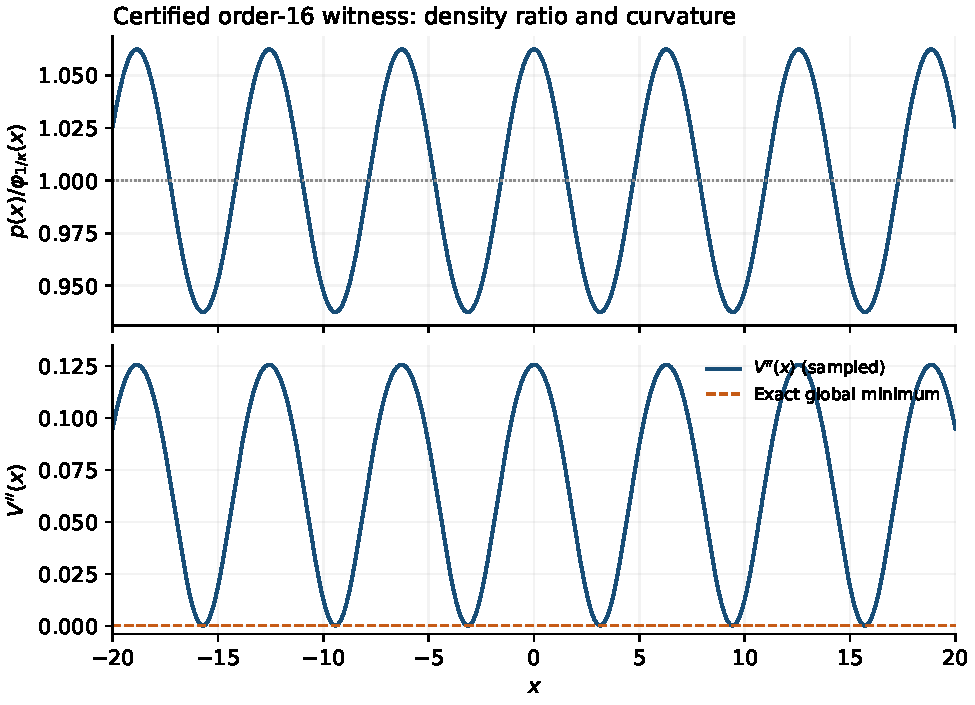
\includegraphics[width=.9\textwidth]{witness16.pdf}
\caption{The explicit order-16 density relative to its Gaussian envelope, and
its potential curvature. The plot is illustrative; the global lower bound
and negative entropy derivative are established by the certificates.}
\end{figure}

\begin{table}[htbp]
\centering
\begin{tabular}{rrc}
\toprule
$m$ & Approximate $S_m(p)$ & Certified sign \\
\midrule
6 & $0.0047085551$ & positive \\
7 & $0.0081424992$ & positive \\
8 & $0.014996902$ & positive \\
12 & $0.28116197$ & positive \\
13 & $0.61425205$ & positive \\
14 & $1.248398$ & positive \\
15 & $1.8940176$ & positive \\
16 & $-0.57212968$ & negative \\
17 & $-14.928482$ & negative \\
18 & $93.05105$ & positive \\
19 & $3571.2182$ & positive \\
20 & $60128.674$ & positive \\
\bottomrule
\end{tabular}
\caption{Derivatives of the same explicit order-16 witness. Displayed values are rounded midpoints; signs are rigorously certified. Full enclosures are in \texttt{certs/witness\_order\_table/}. These are statements about this density only.}
\end{table}



\section{Status and reproducibility}
The current run is ongoing. Exact algebraic certificates establish the
lower-order bounds described above. No exact minimal-order conclusion is claimed.
The authoritative numerical state is in \texttt{checkpoints/campaign\_A.json};
certificates are in \texttt{certs/}. Complete counts and final outcomes will
replace this provisional paragraph after the scheduled campaign.
The code, source literature, and versioned checkpoints are backed up to the
private research repository. Float32 exploration, float64 refinement, and
rigorous interval certification are distinct stages.

\begin{thebibliography}{9}
\bibitem{zou} J. Zou, L. Fan, J. Gao, and J. Wang,
\emph{An Explicit Family of Log-Concave Counterexamples to the Gaussian
Completely Monotone Conjecture}, arXiv:2608.30275 (2026).
\bibitem{gu} Y. Gu and M. Sellke,
\emph{A Counterexample to the Gaussian Completely Monotone Conjecture},
arXiv:2605.11656 (2026).
\bibitem{wang} G. Wang,
\emph{A higher-order Otto calculus approach to the Gaussian completely
monotone conjecture}, arXiv:2408.13957.
\end{thebibliography}
\end{document}
